\chapter{Introduction}


\section{The Transmembrane Protein Problem}
%Kyte and doolittle

The insertion and formation of the unusually orientated \gls{tmh}s and of the more traditional \gls{tmh}s have been shown to be underpinned by complex thermodynamic equilibria \cite{Cymer2014}. \gls{tmh}s have been identified as regulators of protein quality control and trafficking mechanisms, shifting the idea away from \gls{tmh}s broadly simply functioning as anchors \cite{Hessa2011}. The story is not as simple as originally thought. There is a contingency in the field of biological membranes that despite progress over the last decade, there is a still lack of information regarding their structure, assembly, and the behaviour of \gls{tmh}s in the lipid bilayer; the native biological environment of \gls{tmh}s \cite{Ladokhin2015}.


\section{Biological Membrane Composition}

%Something about aysmetry, varies through the tree of life. "before we discuss the membrane proteins, one must consider the biological reason as for why they exist."
%to do:  give specific examples of incredibly useful membrane protiens. Outline that MPs are vital for relaying information and chemistry across the membrane.
\subsection{Lipids of the Membrane}

%At some point the membrane phases should be discussed. Similar to the diagram here perhaps: http://popups.ulg.ac.be/1780-4507/index.php?id=6568
The compartmentalisation of cellular biochemistry is arguably one of the most significant events to have occurred in evolution, and is certainly one of the fundamental prerequisites for life \cite{Koshland2002}.  The proteins that allow life to use this biochemical barrier are perhaps equally important. Together, the lipid bilayer and proteins therein allow complex biochemical systems that facillitate life to exist.

It is critical to understand that the lipid bilayer and the transmembrane $\alpha$ helices are inextricably linked, and often what we observe from the $\alpha$ helices reflect the properties of the much harder to study membranes. The lipid membranes influence the local structure, dynamics, and activity of proteins in the membrane in non-trivial ways \cite{Bondar2010, Bondar2009, Jardon-Valadez2010, Kalvodova2005, Urban2005, White2001, Jensen2004, Henin2014}.%Henin2014. %Add references about the hydrogen bonds (white2005 and another one...) %Perhaps this wedge of citations should be expanded.

There is a rich variety of lipid molecules that make up the biological membranes. The majority of lipids in higher organism membranes are phospholipids, sphingolipids, and sterols. These are composed of a glycerol molecule. Bonded to the glycerol molecule are two hydrophobic fatty acid tail groups, and a negatively-charged polar phosphate group. The polar phosphate group is modeified with an alcohol group. Water entropicly drives the self association of the lipid molecules. In other words the bilayer forms from these phospholipid molecules due to the fierce dissociation between the polar water and the hydrophobic tails. Furthermore the bilayer maximises van der Waals interactions between the closely-packed hydrocarbon chains, which contributes to the stability of the bilayer. This can be seen even in relatively early \gls{md} simulations \cite{Goetz1998}.

\subsection{Differenes in Membrane Compositions}

It has been known for some time that the outer membranes of Gram negative bacteria are asymentric in terms of lipid composition. The outer membranes contain lipopolysccharide, whilst the inner is a mixture of approximately 25 phospholipid types. Adding to the membrane asymmetry composition story, a thorough analysis of residue composition in yeast and human \gls{tmh} regions revealed intra-membrane leaflet composition asymetry in the \gls{er}, but not the Golgi \cite{Sharpe2010}. Furthermore protein\-lipid interactions have been shown to be determinants of membrane curvature \cite{Jensen2004}, and undertake complex orientations and conformations to allow for hydrophobic mismatch \cite{Planque2003}. %the planque reference is messed up. It may need changing with every bib.tex update unless the permannet record is changed.

\subsection{Membrane Potential}
Simply put, membrane potential is the voltage across a membrane. If the membrane is permeable to a certain type of ion, then the ion will experience an electrical pulling force during the diffusion process that will facour the ``preferred'' biological location. This clearly depends on a chemical component involving both the charge and ion concentration gradient.There are various ways of estimating the membrane potential {\it ab initio}.

The Nernst equation can be derived directly from the simplified thermodynamic principles (i) the Boltzmann ditribution, and (ii) a field charge interaction energy \cite{Feiner1994}. It is defined as:

\begin{align*}
{E}_{m} &= \frac{RT}{F}\times \ln { \frac{{c}_{out}}{{c}_{in}} }
\end{align*}

Where charge $Em$ is the membrane potential, $z$ is the ion charge, $c$ is the concentration of an ion in that cell environment.

However, it is rife with caveats caused by the assumptions of the simplified model such as the assumption that ions have point charge, that the potential is not constant throughout the solution and is only measurable at the point of measurement and this can be heavily influenced by, for example, a specific adsorbtion of either part of the redox pair or the competitive adsorption of a supporting ion in solution \cite{Feiner1994}. Therefore one should be cautious to understand the limitations and variability when extrapolating experimentally determined ${E}_{0}$, particularly when using such an idealised model in a biological context. Particulalry, the problems in a biological membrane is that the compartments always  involve multiple ion channels. The Goldman equation aims to solve this problem by accounting for several ions simultaneously:

\begin{align*}
{E}_{m} &= \frac{RT}{F}\times \ln \left(\frac{p_{K^+}.[K^+]_{out} + p_{Na^+}.[Na^+]_{out} + p_{Cl^-}.[Cl^-]_{in}} {p_{K^+}.[K^+]_{in} + p_{Na^+}.[Na^+]_{in} + p_{Cl^-}.[Cl^-]_{out}}\right)
\end{align*}

Where charge $Em$ is the membrane potential, $z$ is the ion charge, $[i]$ is the ion concentration and $p_i$ is the relative membrane permeability for the actual ion

\subsubsection{Organelle Membrane Potential}

Several studies have attempted to quantify the various voltages across the intracellular membranes. Negativity was found in the mitochondrial membrane at 150mV \cite{Perry2011}, and between 75mV to 95mV in the \gls{er} membrane \cite{Qin2011, Worley1994}. No notable membrane potential has been identified in the Golgi \cite{Schapiro2000}.


\section{$\alpha$ Helices in Membranes }
\subsection{The Importance of Transmembrane Proteins}
Membrane bound proteins underpin almost every biological process directly, or indirectly, from photosynthesis to respiration. Integral \gls{tmp} are encoded by around 30\% of the genes in the human genome which reflects their biological importance \cite{Almen2009}. These proteins allow biochemical pathways that traverse the various biological membranes used in life. %citation for drug targets

%This should basically be a summary of Pogozheva, Baeza-delgado, and  Sharpe. Cite examples of direct and indirect accurate prediction methods

%Wong papers on how the sequences contain nuanced signals.

%Function is a result of structure, and here the structure and sequence are supposedly very relatable.
The relationship between the membrane and \gls{tmp}s is underpinned by complex thermondynamic and electrostatic equilibria. Once inserted the protein doesn't leave the membrane as a result of the transmembrane helix being very hydrophobic. This hydrophobicity, and the hydrophobicity of the lipid tails means that they self associate. A better way of describing it is that they fiercely dissociate from the water. The overall $\Delta$G for a transmembrane helix in the membrane is -12kcal${mol}^{\--1}$ \cite{Cymer2014}; the association of the helix in the membrane is typically spontaneous.

\subsection{Transmembrane Helix Sequence Composition}

%WALP and KALP peptides as typical peptides
\begin{figure}[!ht]
\centering
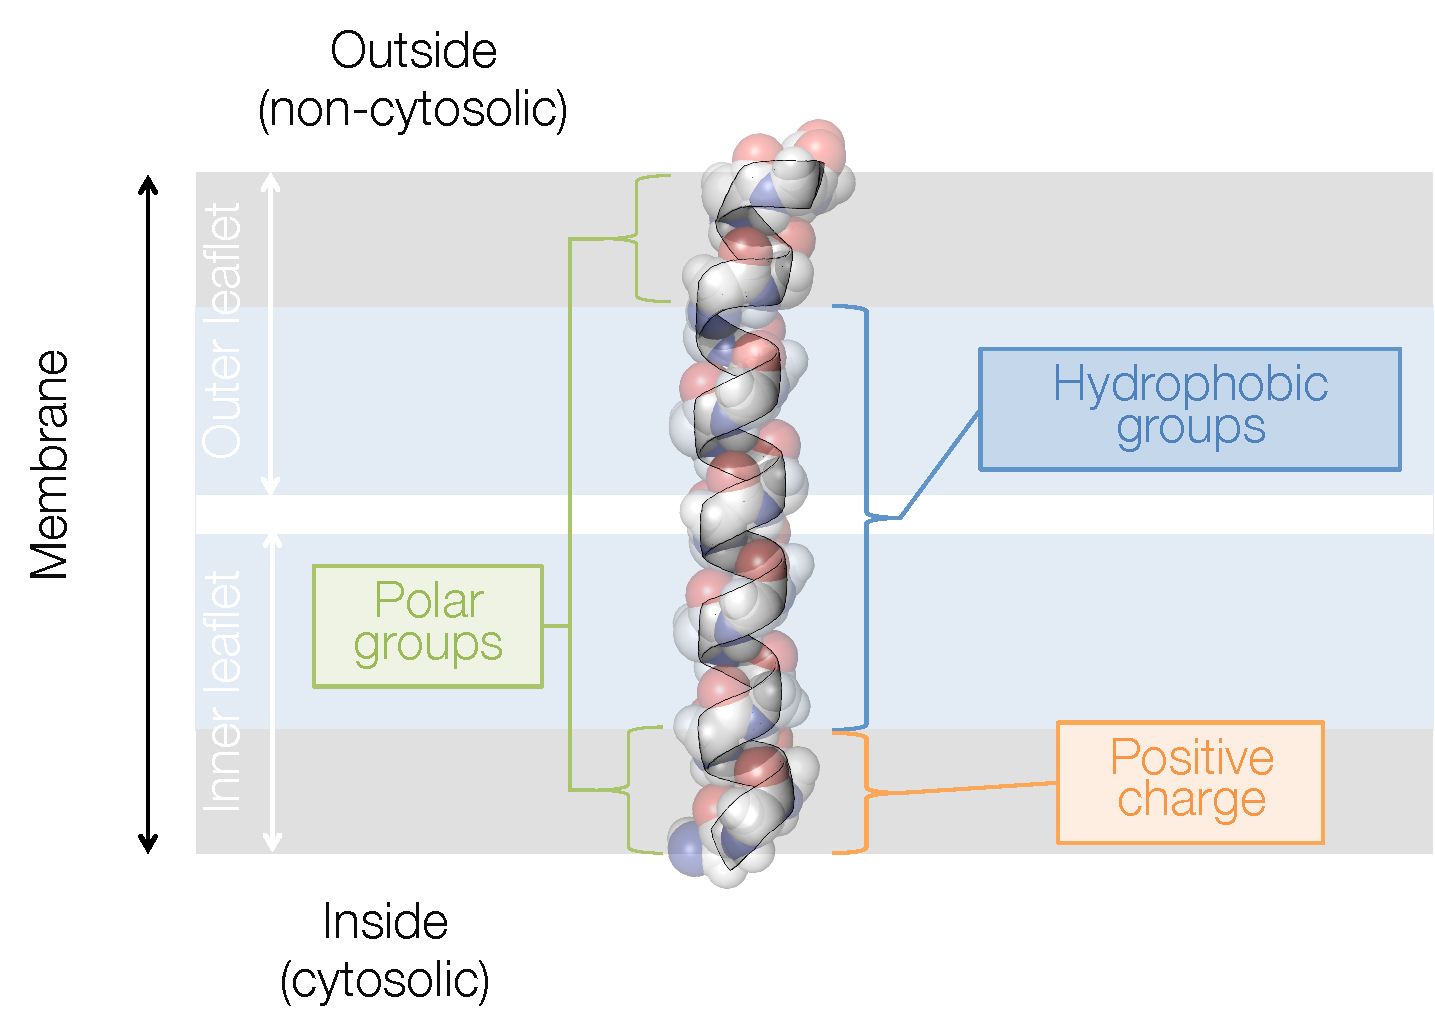
\includegraphics[width=1\textwidth]{Helix_anatomy}
\caption{A cartoon showing the general components of the membrane and a typical \gls{tmh}. The example used here for illustrative purposes is transmembrane region of tetherin (PDB 2LK9) \cite{Skasko2012}. Dark grey areas denote the area of lipid head groups. The residues found in these areas are often described as flanking regions, and are often in contact with the aqueous interface of the membrane. The helix core is mostly composed of hydrophobic residues. More recently the hydrophobic group region has been associated with cell localisation and a broad range of biochemical functions \cite{Junne2010, Wong2012}. Although the regions labelled here generally hold true in terms of the statistical distribution of polar, non-polar, and charged groups, it is by no means absolute laws and many proteins break these ``rules'' \cite{Sharpe2010, Baeza-Delgado2013, Pogozheva2013}. Note that the definition of a \gls{tm} $\alpha$-helix is not entirely clear; how far the helix rises into the water-interface region to qualify as a \gls{tmh} for example \cite{VonHeijne2006}.}
\label{fig:helixcartoon1}
\end{figure}


% Figure: A cartoon depicting various problematic, yet biologically observed topologies and lengths that the alpha helices can adopt. From left to right: a typical and traditional \gls{tmh}, an exceptionally long \gls{tmh}, a \gls{tmh} that lies flat in the interface region, a kinked helix that enters and exits the bilayer on the same leaflet, a \gls{tmh} that is not long enough to span the entire membrane. Note that these exceptional formations present a challenge for topology predictions of the loop regions.}


Properties that can be analysed by bioinformatics, the sequence complexity and hydrophobicity, of the \gls{tmh} have been used to predict the role of the \gls{tmh} as either functional or structural, and as a discrete cluster from other SCOP annotated helices \cite{Wong2012}. Those findings demonstrated that the sequence of the \gls{tmh} holds valuable information regarding biological roles, and forms the basis of our interest in the link between the polarity of a helix and functional activity beyond structural anchorage.

The language used to describe \gls{tmh}s varies somewhat across the literature, primarily due to a changing understanding of \gls{tmh} general structure and relevance to function over the last 15 years or so. There is a general composition of a \gls{tmh} despite specific protein and membrane constraints \cite{Sharpe2010}.

%This paragraph should certainly be changed to the updated one from the manuscript.
A study by Baeza-Delgado {\it et al.} from 2013 \cite{Baeza-Delgado2013} looked at \gls{tmh}s in 170 integral membrane proteins from a manually maintained database of experimentally confirmed \gls{tmp}s; MPTopo \cite{Jayasinghe2001}. The group examined the distribution of residues along the \gls{tmh}s. As expected, half of the natural amino acids are equally distributed along Transmembrane (TM) helices whereas aromatic, polar, and charged amino acids along with proline are biasedly near the flanks of the TM helices \cite{Baeza-Delgado2013}. It has been noted that transitions between the polar and non-polar groups at the ends of the hydrophobic core occur in a more defined edge on the cytoplasmic side than at the extracytoplasmic face when counting from the middle of the helix outwards \cite{Baeza-Delgado2013}. This is probably reflecting the different lipid composition of both leaflets of biological membranes \cite{Baeza-Delgado2013}. A larger previous study using 1192 human and 1119 yeast predicted \gls{tmh}s that were not structurally validated further explored the difference in \gls{tmh} and leaflet structure by exploiting the evolutionarily conserved sequence differences between the \gls{tmh} in the inner and outer leaflets \cite{Sharpe2010}. \gls{tmh}s from vertebrates and invertebrates were found to be reasonably similar compositionally. The differences in consensus \gls{tmh} structure implies that there are general differences between the membranes of the golgi and \gls{er}. The abundance of serines in the region following the lumenal end of golgi TMDs probably reflects the fact that this part of many golgi enzymes forms a flexible linker that tethers the catalytic domain to the membrane \cite{Sharpe2010}.

\subsubsection{The ``Positive-Inside'' Rule}

Two publications by von Heijne coined the ``Positive-Inside'' rule demonstrated the practical value of positively charged residue sequence clustering in topology prediction of \gls{tmh}s in bacteria \cite{VonHeijne1989,VonHeijne1992}. It was clearly defined and shown that positively charged residues more commonly were found on the ``inside'' of the cytoplasm rather than the periplasm of {\it E. coli}. More recently still large scale sequence analysis of \gls{tmh}s from different organelle membrane surfaces in eukaryotic proteomes, show the clustering of positive charge being cytosolic \cite{Sharpe2010, Baeza-Delgado2013, Pogozheva2013}.

\subsubsection{The Aromatic Belt}

 Tyrosine and tryptophan residues commonly are found at the interfacial boundaries of the \gls{tmh} and this feature is called the ``aromatic belt'' \cite{Hessa2005, Granseth2005, Sharpe2010, Baeza-Delgado2013, Nilsson2005}. Not all aromatic residues are not found in the aromatic belt; phenylalanine has no particular preference for this region \cite{Granseth2005, Braun1999}. However it still remains unclear if this is to do with anchorage or translocon recognition \cite{Baeza-Delgado2013}.

%More than one explanation has been proposed for the physical and/or chemical basis for the strong preference of aromatic residues to reside in the membrane-water interface region. The Tyrosine side chain is a six-membered aromatic ring with an –OH group attached. Tryptophan has two aromatic rings that are fused into one large hydrophobic ring-structure. Phenylalanine, although aromatic, is completely hydrophobic, and is found in the transmembrane part rather than the interfacial parts of MPs. The classical explanation for the preference of Tyrosine and Tryptophan to reside in the interfacial regions is their dipolar character. The side chain must simply seek a compromise. This can be achieved by burying the aromatic ring close to, or within, the hydrophobic core, while the hydrophilic part can interact with the polar lipid head-groups at the interface. Other factors such as the aromaticity, size, rigidity and shape of Tryptophan, rather than its dipolar character, has also been suggested as the primary reasons for its interfacial preference [91]. Perhaps, as suggested by You et al., it is a balance of all these forces that explains the interfacial preference of Tyrosine and Tryptophan [91

\subsubsection{Snorkeling}

Broadly speaking, transmembrane helices are non-polar. However some contain polar and  charged residues in the helix itself. Whilst this might seem thermodynamically unstable at first glance, a molecular dynamic feature called the ``snorkel'' effect explains in part how this is possible \cite{Chamberlain2004, Strandberg2003}. Simply put, the snorkelling effect involves the long flexible side chain of leucine reaching the water interface region to interact with the polar headgroups of the bilayer even when the $\alpha$ helix backbone is pulled into the hydrophobic layer \cite{Krishnakumar2007}. This has also been suggested to allow helices to adapt to varying thicknesses of the membrane \cite{Kandasamy2006}.

\section{Biogenesis of Transmembrane Proteins}
%Depth of secretion pathway (talk about translocons in depth here) & outline post-translational insertion
\subsection{Translocation}
The ``inside'' was an imprecise term used to indirectly refer to the cytoplasmic space. To understand why the cytoplasm is the key part, one must recall how the membranes are synthesised and localised throughout the cell.

\subsection{Tail-Anchored Proteins Post Translationally Insert}

Tail anchored proteins are a topologically distinct class of intracellular proteins defined by their single carboxy-terminal transmembrane domain with a cytosolic facing amino-terminus. Tail anchored proteins are involved in a range of key cellular functions including protein translocation and apoptosis. Additionally, within the tail anchored class of proteins are a set of vesicle fusion proteins called \gls{snare} proteins. There is biomedical interest in \gls{snare} drug delivery mechanisms. \gls{snare}s can fuse liposomes containing various drug payloads into the membrane.

Notably, known \gls{snare} transmembrane helices are highly hydrophobic even compared to other tail anchored transmembrane helices.

\subsection{Translocon Independent Membrane Insertion}
%move on to case studies involving spontaneous insertion?
Signal anchored proteins, proteins that contain a single hydrophobic segment that serves as both a mitochondrial targeting signal and a membrane anchor, as well as tail anchored proteins have been shown to be able to spontaneously insert into the membrane indepently from the translocon \cite{Elisa2012, Lan2000, Colombo2009}.

It is postulated that there are electrostatic factors in the flanking regions that contribute to this spontaneous membrane insertion. Our experimental collaborators in Stephen High’s group are interested in a small group of tail anchored proteins that have very polar transmembrane domains and are capable of liposome membrane insertion without insertion machinery, also known as spontaneous insertion. They have found that chimeric synaptobrevin, one of the first identified \gls{snare} proteins, is capable of spontaneous insertion if it’s tail anchor domain is replaced by the transmembrane domains belonging to a protein of known spontaneously inserting domains. Their studies have moved the focus of spontaneous insertion away from the loop regions and onto the biophysicochemical factors of the TMH itself. The idea that \gls{snare} proteins are modular, and capable of spontaneous insertion has significant implications for both biomedical application in liposome based drug delivery and can aid future research for testing complex biological molecular networks \cite{Allen2013, Nordlund2014}.

\section{Choice of Hydrophobicity Values}
\subsection{An Overview of the Different Scales}
Throughout this thesis several scales are used to evaluate and estimate hydrophobic values of peptides. All the scales aim for quantifying the hydrophobic values of each residue. There are several key differences in their methodology, assumptions, and aims. Crucially this results in slightly different scores for some residues. Because of this, it's preferable, and typical amongst the literature, to use several scales to verify the patterns observable in one scale. Notably, one of the classic scale, Kyte \& Doolittle Hydropathy Scale shows striking similarity to the modern Hessa's Biological Hydrophobicity Scale, and that generally the ``better'' scales count proline as hydrophilic, and focus on helix recognition rather than amino acid analogues \cite{Peters2014}. Ultimately, all the scales are attempting to allow estimation of ${\Delta G}_{whf}$; the free energy of a folded helix ({\it f}) from the water ({\it w}) into the membrane core ({\it h}). This free energy measurement is regarded as being currently experimentally inaccessible \cite{Cymer2014}.

%Figure here showing what delta G is on about
%Also a note on arrest peptides

\subsubsection{Kyte \& Doolittle Hydropathy Scale}
A scale based on the water\---vapour transfer free energy and the interior-exterior distribution of individual amino acids \cite{Kyte1982}.

\subsubsection{Hessa's Biological Hydrophobicity Scale}
This is arguably the most biologically relevent scale \cite{Peters2014}. The scale is based on an experimental method where the free energy exchange during recognition of designed polypeptide helices by the endoplasmic reticulum Sec61 translocon occured \cite{Hessa2005}. These measurements were then used to calculate a “biological hydrophobicity scale.”

\subsubsection{White and Wimley Octanol \--- Interface Whole Residue Scale}
This scale is calculated from two other scales; the octanol scale, and the interface scale \cite{White1999}. This scale is fundamentally based on the partitioning of host-guest pentapeptides (acetyl-WL-X-LL-OH) and another set of peptides (AcWLm) between water and octanol, as well as water to \gls{popc} .


\subsubsection{The Eisenberg Hydrophobic Moment Consensus Scale}
The Eisenberg scale is a consensus scale based on the earlier scales from Tanford \cite{Nozaki1971}, Wolfenden \cite{Rose1993}, Chothia \cite{Chothia1976}, Janin \cite{Janin1979}, and the von Heijne scale \cite{VonHeijne1979}. The scales are normalized according to serine \cite{Eisenberg1984}. The automatic TRANSMEM annotation currently used in Uniprot is according to TMHMM \cite{Krogh2001}, Memsat \cite{Jones2007}, Phobius \cite{Kall2004} and the hydrophobic moment plot method of Eisenberg and coworkers \cite{Eisenberg1984}.


\section{A Brief History of Transmembrane Proteins in Science}
\subsection{Earliest Evidences of Compartmentalisation}
%To get started https://en.wikipedia.org/wiki/History_of_cell_membrane_theory
%A group linking computational biophycs http://www.ks.uiuc.edu/History/membrane/

%Some waffle about Hooke

\subsection{Early Models of the Bilayer}
%Gorter & Grendel
%Danielli and Davson http://biology.stackexchange.com/questions/20264/why-was-the-davson-danielli-model-rejected/24051#24051

\subsection{The Rise of Crystallography}
%first crystals in the membrane

Because of the experimental hinderence, the story of transmembrane proteins has been relatively slow to emerge. In the 1990s and early 2000s the story was seemingly uncomplicated. There were membrane-spanning bundles of non-polar α-helices of roughly 20 residues length, with a consistent orientation of being perpendicular to the membrane surface. Since the mid-2000s the elucidation of many more intramembrane helix structures implied a far richer variety of transmembrane helices existed than previously thought, with a range of orientations and intra-membrane biophysical variations. Although the simple helices are broadly prevelant, hundreds of high quality membrane structures have elucidated that \gls{tmh}s can adopt a plethora of lengths and orientations within the membrane. \gls{tmh}s are capable of partial spanning of the membrane, spanning using oblique angles, and even lying flat on the membrane surface \cite{VonHeijne2006, Elofsson2007} (Figure \ref{fig:helixcartoon1}). Over the last decade, Nanodiscs have been routinely used to much more easily obtain crystal structures. Nanodiscs overcome some of the major challenges caused by the hydrophobic helices, and a more faithful representation of the biological membranes than alternative model membranes like liposomes \cite{Borch2009}. %Figure for Nanodisc
%Development of Nanodiscs

%At the time of writing, how many in PDB.

\section{Aims of This Thesis.}

\begin{enumerate}
  \item Negative not inside rule
  \item \gls{gpi} project
  \item \gls{snare} and \gls{ta} project
  \item Good and bad helices
\end{enumerate}
